\documentclass[12pt]{article}
\usepackage[utf8]{inputenc}
\usepackage{graphicx} % This package is used to render figures
\usepackage{booktabs} % This package is used to make tables look nice
\usepackage{tikz}  % This package can be used to make graphs (i.e., nodes with edges)
\usepackage{parskip}
\usepackage{algorithm} % This package is used to render algorithms
\usepackage{amsmath} % These packages are for math symbols
\usepackage{amsfonts}
\usepackage{amssymb}

\usepackage[noend]{algpseudocode}
\usepackage{url}

\graphicspath{{./figures}} % This is where you find the figures

\usepackage{times}
\usepackage{helvet}
\usepackage{courier}
\usepackage{listings}


% The file iccc.sty is the style file for ICCC proceedings.
%

\lstdefinestyle{mystyle}{
    language=Python,
    basicstyle=\ttfamily,
    keywordstyle=\color{blue},
    commentstyle=\color{green!50!black},
    stringstyle=\color{red},
    showstringspaces=false,
    numbers=left,
    numberstyle=\normalfont,
    numbersep=5pt,
    breaklines=true,
    breakatwhitespace=true,
    tabsize=2,
    captionpos=b
}


\title{Report on Traveling Salesperson}
\author{Sabal Subedi \\
Master's in Computer Science\\
Idaho State University\\
Pocatello, ID, 83209  USA\\
sabalsubedi@isu.edu\\
}               


\begin{document}

\maketitle

\begin{abstract}
This project report summarizes the use of the branch and bound algorithm to solve the traveling salesperson problem.
\end{abstract}
    
\section{Introduction}
Branch and bound is a method for solving optimization problems by breaking them down into smaller sub-problems and using a bounding function to eliminate sub-problems that cannot contain 
the optimal solution. The algorithm depends on efficient estimation of the lower and upper bounds of regions/branches of the search space. If no bounds are available, the algorithm degenerates to an exhaustive search.
\\
The algorithm explores branches of the tree, which represent subsets of the solution set. Before enumerating the candidate solutions of a branch, the branch is checked against upper and lower estimated 
bounds on the optimal solution, and is discarded if it cannot produce a better solution than the best one found so far by the algorithm.
\newpage
\section{Pseudocode and Asymptotic Analysis}

\subsection{Pseudocode for branch and bound algorithm}
\begin{lstlisting}[style=mystyle]
    def branchAndBound(self, time_allowance=60.0):
        results = {"pruned": 0, "total": 0, "max": 0, "count": 0}
        cities = self._scenario.getCities()
        ncities = len(cities)
        foundTour = False
        # use priority queue to keep track of next subproblem to search
        priority_queue = []
        # dictionary mapping priority hashing to sub problem
        priority_dict = {}
        cost, matrix = self.create_initial_matrix(cities)
        # initial BSSF using greedy approach
        greedy_bssf = self.greedy()
        if greedy_bssf["cost"] != np.inf:
            foundTour = True
            bssf = BSSF(
                greedy_bssf["cost"], [city._index for city in greedy_bssf["soln"].route]
            )
        else:
            bssf = BSSF(np.inf, None)
        start_time = time.time()
        timed_out = False
        initial_node = 0
        cur_path = [initial_node]
        initial_problem = SubProblem(cost, matrix, cur_path)
        results["total"] += 1
        # update the priority queue
        self.add_to_queue(initial_problem, priority_queue, priority_dict)
        while len(priority_queue) != 0:
            # sort the priority queue
            priority_queue.sort(reverse=True)
            cur_problem_score = priority_queue.pop()
            cur_problem = priority_dict[cur_problem_score]
            for j in range(ncities):
                # Check timeout
                if time.time() - start_time > time_allowance:
                    timed_out = True
                    break
                # expand the subproblem
                problemChild = self.expand_subproblem(cur_problem, j, results)
                if problemChild is None:
                    continue
                results["total"] += 1
                if len(problemChild.path) == ncities:
                    if (
                        problemChild.matrix[problemChild.path[-1], problemChild.path[0]]
                        != np.inf
                    ):
                        foundTour = True
                        problemChild.cost += problemChild.matrix[
                            problemChild.path[-1], problemChild.path[0]
                        ]
                        # update the BSSF
                        if problemChild.cost < bssf.cost:
                            results["count"] += 1
                            bssf.cost = problemChild.cost
                            bssf.route = problemChild.path
                            continue
                        # prune the child
                        else:
                            results["pruned"] += 1
                    else:
                        results["pruned"] += 1
                elif problemChild.cost >= bssf.cost:
                    results["pruned"] += 1
                else:
                    self.add_to_queue(problemChild, priority_queue, priority_dict)
                    if len(priority_queue) > results["max"]:
                        results["max"] = len(priority_queue)
            # check timeout
            if timed_out:
                break
        citiesPath = [cities[index] for index in bssf.route]
        bandbSolution = TSPSolution(citiesPath)
        end_time = time.time()
        # update the result
        results["cost"] = bandbSolution.cost if foundTour else math.inf
        results["time"] = end_time - start_time
        results["soln"] = bandbSolution
        return results
    \end{lstlisting}
\newpage

\noindent\textbf{Time complexity and space complexity} 
\begin{enumerate}
    \item to add cities in priority queue takes $O(1)$ time and $O(n)$ spaces
    \item outer loop iterates over all the cities $O(n)$ times
    \item to sort and update the cities in priority queue it takes $O(n \log n)$ times and $O(n)$ spaces 
    \item inner loop iterates over all the expanded state $O(n!)$ times
    \item while expanding the subproblem, generating successor states takes $O(n!)$ times and $O(n!)$ 
    spaces and to compute the reduced cost matrix it takes $O(n^2)$ times and $O(1)$ space
    \item to update the results it takes $O(n)$ times and $O(n)$ spaces    
\end{enumerate}
\begin{equation} % You should use descriptive variable names (not eq1)
\begin{split}
    Time\_complexity =& O(1) + O(n) * (O(n \log n) + O(n!) * (O(n!) + O(n^2) + O(n))) \\ 
    &\approx O(n!) \\
    Space\_complexity =& O(n) + O(n) * (O(n) + O(n!) + O(n!) + O(1) + O(n)) \\
    &\approx O(n!)
\end{split}
\end{equation}

\newpage

\subsection{Pseudocode for greedy algorithm}
\begin{lstlisting}[style=mystyle]
    def greedy(self, time_allowance=60.0):
        cities = self._scenario.getCities()
        cost, matrix = self.create_initial_matrix(cities)  # extract initial cost
        results = {
            "cost": math.inf,
            "time": 0.0,
            "soln": None,
            "count": 0,
            "max": None,
            "total": None,
            "pruned": None,
        }
        start_time = time.time()
        # Iterate over possible starting nodes
        for initial_node in range(len(cities)):
            greedy_matrix = matrix.copy()
            greedy_cost = cost
            path = [initial_node]

            while len(path) != len(cities):
                # Check timeout
                if time.time() - start_time >= time_allowance:
                    return results

                min_val, col_index = self.find_next_city(greedy_matrix, path)
                # No valid path found
                if min_val == np.inf:
                    break
                self.update_greedy_matrix(greedy_matrix, col_index, path)
                greedy_cost += min_val
            # complete tour found
            else:
                greedy_cost += greedy_matrix[path[-1], initial_node]
                cities_path = [cities[i] for i in path]
                solution = TSPSolution(cities_path)
                if solution.cost < results["cost"]:
                    results["cost"] = solution.cost
                    results["time"] = time.time() - start_time
                    results["soln"] = solution
                    results["count"] = 1
        return results
    \end{lstlisting}

\noindent\textbf{Time complexity and space complexity}
\begin{enumerate}
    \item outer loop iterates over each possible starting node which takes $O(n)$ times
    \item inner loop iterates over all cities to find the next city with minimum cost edge, taking $O(n)$ times
    \item to find next city with minimum cost edge takes $O(n)$ times
    \item to update the greedy matrix takes $O(1)$ times
    \item to store greedy matrix takes $O(n^2)$ space 
\end{enumerate}
\begin{equation} % You should use descriptive variable names (not eq1)
\begin{split}
    &Time\_complexity = O(n) * O(n) * (O(n) + O(1)) \approx O(n^3)\\
    &Space\_complexity = O(n^2) 
\end{split}
\end{equation}

\newpage

\subsection{Pseudocode for helper functions}
\begin{lstlisting}[style=mystyle]
    # function to expand subproblem
    def expand_subproblem(self, subProblem, col, results):
        if subProblem.matrix[subProblem.path[-1], col] == np.inf:
            return None

        matrix_copy = subProblem.matrix.copy()
        matrix_copy[subProblem.path[-1]] = np.inf
        matrix_copy[:, col] = np.inf
        matrix_copy[col, subProblem.path[-1]] = np.inf

        reductionCost = self.reduce_cost_matrix(matrix_copy)

        new_cost = (
            reductionCost
            + subProblem.cost
            + subProblem.matrix[subProblem.path[-1], col]
        )
        new_path = subProblem.path.copy()
        new_path.append(col)
        return SubProblem(new_cost, matrix_copy, new_path)
    \end{lstlisting}
\newpage
\begin{lstlisting}[style=mystyle]
    # function to compute reduced cost matrix
    def reduce_cost_matrix(self, matrix):
    lower_bound = 0
    for i in range(len(matrix)):
        row_min = min(matrix[i, :])
        if row_min != np.inf:
            matrix[i] -= row_min
            lower_bound += row_min
    for j in range(len(matrix)):
        col_min = min(matrix[:, j])
        if col_min != np.inf:
            matrix[:, j] -= col_min
            lower_bound += col_min
    return lower_bound
\end{lstlisting}

\begin{lstlisting}[style=mystyle]
    # function to compute initial matrix
    def create_initial_matrix(self, cities):
        initMatrix = np.full((len(cities), len(cities)), np.inf)
        reductionCost = 0
        for i, city_i in enumerate(cities):
            for j, city_j in enumerate(cities):
                if i != j:
                    initMatrix[i, j] = city_i.costTo(city_j)
        reductionCost = self.reduce_cost_matrix(initMatrix)
        return reductionCost, initMatrix
\end{lstlisting}

\begin{lstlisting}[style=mystyle]
    # function to add items in queue
    def add_to_queue(self, subProblem, priority_queue, priority_dict):
        hash_value = subProblem.cost / len(subProblem.path)
        priority_queue.append(hash_value)
        priority_dict[hash_value] = subProblem
    \end{lstlisting}

\newpage
\noindent\textbf{Time complexity and space complexity} \\
\begin{enumerate}
    \item to expand the subproblem it takes $O(n^2)$ times \\
    and $O(n^2)$ space to copy matrix
    \item to compute the reduced cost matrix it takes $O(n^2)$ times \\
    and $O(n^2)$ space
    \item to compute the initial cost matrix it takes $O(n^2)$ times \\
    and $O(n^2)$ space
    \item to add items in queue it takes $O(1)$ time and $O(1)$ space
\end{enumerate}

\newpage

\section{Observations and Results}

\subsection{Observation Table}
\begin{figure}[h]. % the 't' asks LaTeX to put this figure on the top of the page   
    \begin{center}
      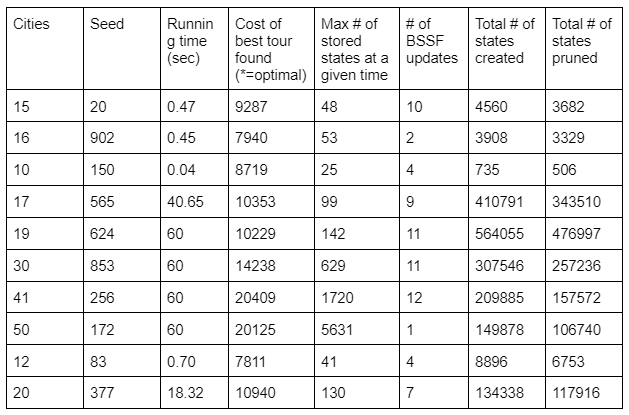
\includegraphics[width=0.90\linewidth]{figures/table.png} 
      \caption{Observation table with different number of cities and seed}\label{fig:table}
    \end{center}
  \end{figure}
\noindent In the figure (in figure 1), the seed represents the randomness, cities represents the number of cities, running time indicates time taken by program to compute branch and bound algorithm, cost of best tour indicates the optimal cost, 
max of stored states represents the number of item in priority queue, total number of states created and total number of states pruned. \\
The observation table reflects the exponential nature of the TSP problem i.e. the problem size increases as the number of states increases factorially. The number of 
pruned states also increases as the problem size increases. The algorithm effectively eliminates suboptimal paths using the lower bound criteria. This helps to reduce the 
the search space making algorithm more efficient.\\
However, we can still see the increment in time taken to solve the problem with increased problem size because increased problem size 
also increases the number of states to explore. This indicates that, the time complexity grows rapidly with problem size due to the factorial growth in the number of states to explore.

\textbf{Mechanism for state space search}\\
I used the branch and bound algorithm to solve the TSP problem. Unlike the brute force method, this method is effective. First, BSSF is computed using the greedy approach, then the state is branched into multiple smaller subproblems.
For each subproblem, the lower bound is computed and then compared with the initial BSSF. All those subproblems with lower bound greater than the BSSF will be pruned. In this way, the algorithm 
works in two steps: branching the problem and bounding the subproblems. \\
To get the solution more efficiently, geting the BSSF using greedy approach potentially reduces the search space. Similarly, the lower bound criterion helps to eliminate the suboptimal paths early which 
reduces the number of states to explore. Also the use of priority queue helps to identify the potential subproblem that might give optimal solution. The cities (subproblems) are sorted in
 the priority queue which helps the program to choose the best subproblem and eventually get the optimal solution.


\subsection{Results and Analysis}
\begin{enumerate}
    \item Priority queue - For insertion and removal of item from priority queue, it takes $O(n \log n)$ time and these operations are performed for every expanded state, which happens at most $O(n!)$ times. Thus, total time complexity is $O(n!)$ and space complexity is $O(n!)$
    \item Search States - For generating the successor states, we need to iterate through every cities, which is $O(n)$ times and
    the operation is performed for every state, which happens at most $O(n!)$ times. Thus, total time complexity is $O(n!)$ 
    \item Reduced Cost Matrix - To update the reduced cost matrix, it takes $O(n^2)$ times and space complexity is $O(n^2)$
    \item BSSF Initialization - We use greedy approach i.e. choose the tour based on the minimal edge cost from the starting city. So, the time and space complexity is $O(n^2)$
    \item Expanding on SearchState into others - Expanding the subproblem involves generating successor states and updating the priority queue. So, the time complexity is $O(n!)$
\end{enumerate}
\noindent The data structure used to represent the states are matrix. \\ \\
The priority queue data structure I used is the list. Using the subproblem, we compute the hash value and it is added to priority dictionary as key and value pair.\\ \\
To initialize the BSSF, I used the greedy approach. The starting city is selected randomly then the next city is chosen based on the next closest edge of the neighboring cities.


\section{Conclusion}
I coded the branch and bound algorithm to solve the traveling salesperson problem. I used the greedy approach to calculate the initial BSSF. The program computes the inital BSSF 
and checks the criteria i.e compares lower bound against sub optimal paths and prune the state. \\
The branch and bound algorithm works in two steps: expand the subproblems and then enforcing 
certain boundaries i.e. bound,  the program reflects the exponential nature of the TSP problem. As the problem size increases, the number of possible permutations increases factorially.
Then, the program prunes the states that maynot lead to the optimal solution.


\end{document}